\section{Data Analysis with De-Noising}

In this section we compare results from analysis of background merged data sample with files that were de-noised prior to running through CLAS12 reconstruction software. The comparison is done for data samples with different luminosities (namely $45~nA$, $95~nA$ and $150~nA$). The data for raw sample and de-nosied sample are processed with same settings of CLAS12 reconstruction software and the tracks reconstructed in each sample are analyzed.

\subsection{Luminosity dependence}

The track reconstruction efficiency is calculated according to Eq.~\ref{eq::eff} for positive and negative charged particles. The results are shown on Figure~\ref{lscan::conv_dn}. 

\begin{figure}[!h]
\begin{center}
 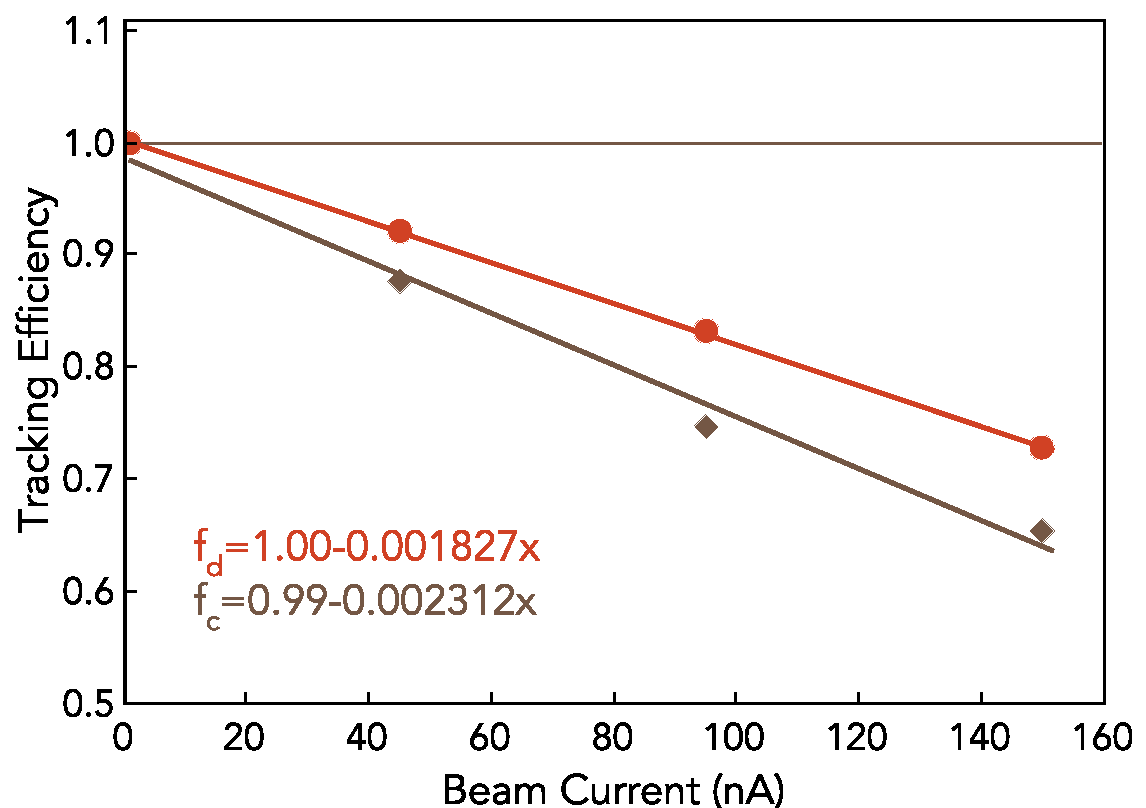
\includegraphics[width=3.1in]{images/figure_lscan_pos.pdf}
 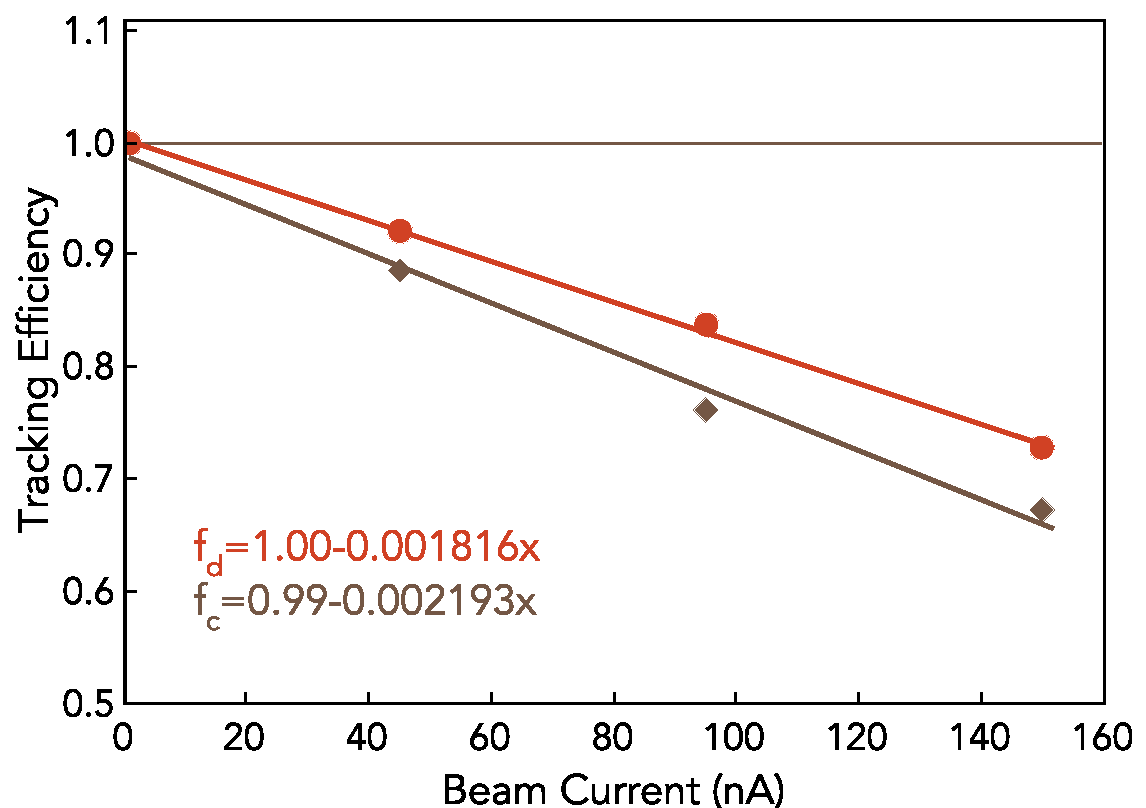
\includegraphics[width=3in]{images/figure_lscan_neg.pdf}
\caption {Tracking efficiency as a function of luminosity (beam current) for positive (a) and negative particle (b).  The efficiency is shown for
conventional algorithm running on background merged files (diamonds), and on files with merged background then de-noised with AI (circles).}
 \label{lscan::conv_dn}
 \end{center}
\end{figure}

As can be seen from the figure the number of reconstructed hadron-electron pairs relative to reconstructed electrons is higher for de-noised data sample compared to the raw data sample. This is due to increased number of clusters reconstructed by conventional clustering algorithm in de-noised data samples. Detailed studies of cluster reconstruction efficiency are performed 
in our studies of neural network paper~\cite{Thomadakis:2022zcd}. 
The result show that the slope of efficiency degradation as a function of luminosity is significantly improved in de-noised data sample. 
It is worth noting that at $75~nA$ the de-noised data sample track reconstruction efficiency is same as for the $45~nA$ when reconstructing raw data sample (without de-noising). This implies that experiment can run at effectively at $75~nA$, collecting data twice faster while maintaining the same track reconstruction efficiency, which will lead to higher experimental significance in measured observables.

\subsection{Physics Impact}

The processed data was also evaluated to extract physics observables from both data sample to discern the impact on physics for de-noising algorithm. As mentioned before, the data selected from Pythia simulation was for the final state $H(e,e^\prime\pi^+\pi^-p)X$ containing exactly three charged particles. From this sample the missing mass distribution of $H(e,e^\prime\pi^+\pi^-)X$ is analyzed showing a peak around proton mass where the selected reaction is inclusive $\rho$ meson production and some background (above proton mass) where other reactions  are present (with missing neutral particles).

\begin{figure}[!h]
\begin{center}
  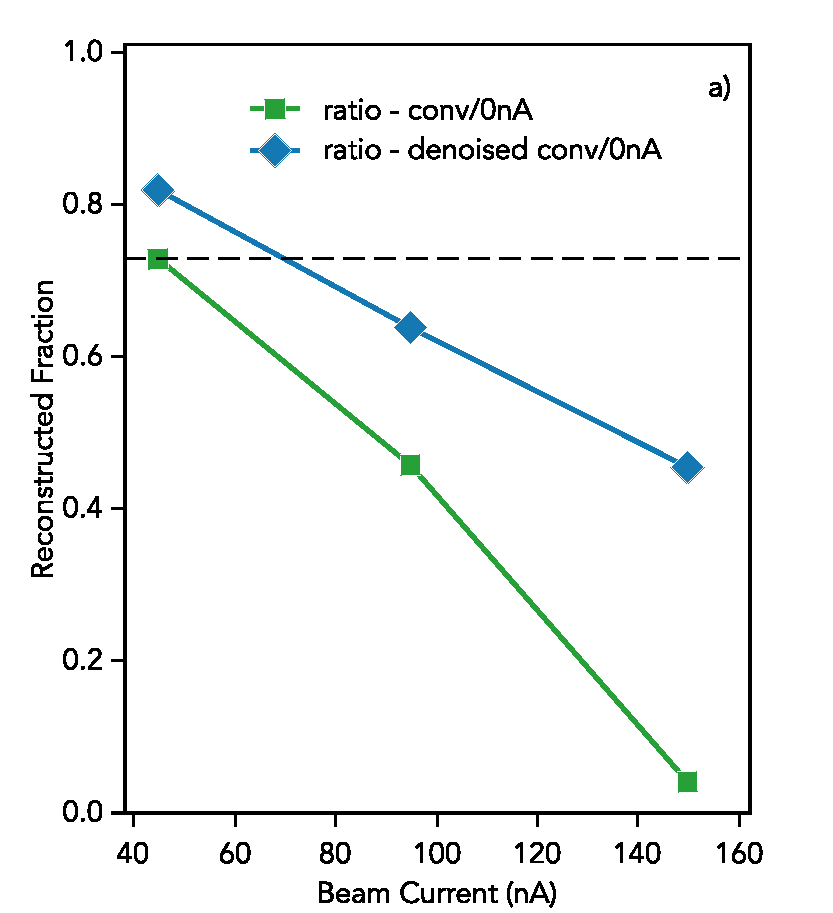
\includegraphics[height=3.1in]{images/graph_mxepipi_dn.pdf}
 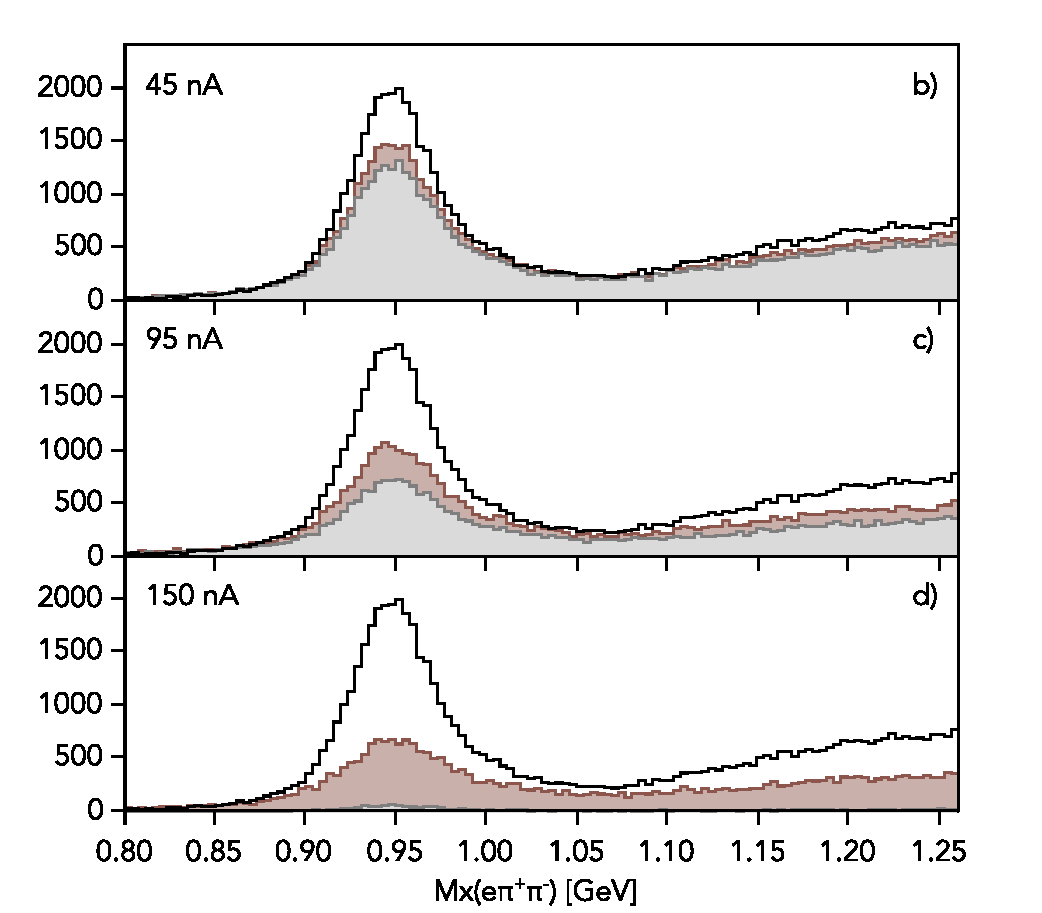
\includegraphics[height=3.1in]{images/plots_mxepipi_dn.pdf}
\caption {a) Number of reconstructed protons from missing mass of $H(e \rightarrow e^\prime \pi^+\pi^-)X$ 
for background merged data set reconstructed with conventional tracking (squares) compared to de-noised data sample 
reconstructed with conventional algorithm (diamonds) for $45~nA$, $95~nA$ and $150~nA$. b), c) and d) reconstructed 
missing mass distributions for background merged data set reconstructed with conventional tracking (filled histogram) and
de-noised data sample reconstructed with conventional algorithm (solid line histogram). Missing mass distribution for
data sample before background merging ($0~nA$) is shown (circles) for reference. }
 \label{physics::conv_dn}
 \end{center}
\end{figure}

In Figure~\ref{physics::conv_dn} the results of analysis are shown, where the missing mass distribution $H(e,e^\prime\pi^+\pi^-)X$ is shown for all different beam currents. In panels b) ,c) and d) the histograms show relative reconstructed distributions. The graph with points shows the missing mass reconstructed by conventional tracking algorithm before any background is mixed in for reference. The filled histogram shows missing mass distribution reconstructed from background merged files with conventional algorithm. The solid line histogram is the missing mass distribution reconstructed by conventional algorithm after the background merged file is processed with de-noising neural network to remove nose hits.
The summary of number of protons under the missing mass distribution relative to original (no background merged) distribution is presented in Figure~\ref{physics::conv_dn} a). It can be seen from the figure that conventional algorithm reconstructs more tracks after de-noising the data. The number of reconstructed proton final states at $75nA$ from de-noised data is equal to number of reconstructed final states at $45nA$ when using conventional track reconstruction algorithms.  Conducting experiments with higher incident beam current allows to accumulate necessary statistics for proposed experiments in significantly less time, leading to huge savings in operating accelerator.

%\begin{figure}[!ht]
%\begin{center}
 %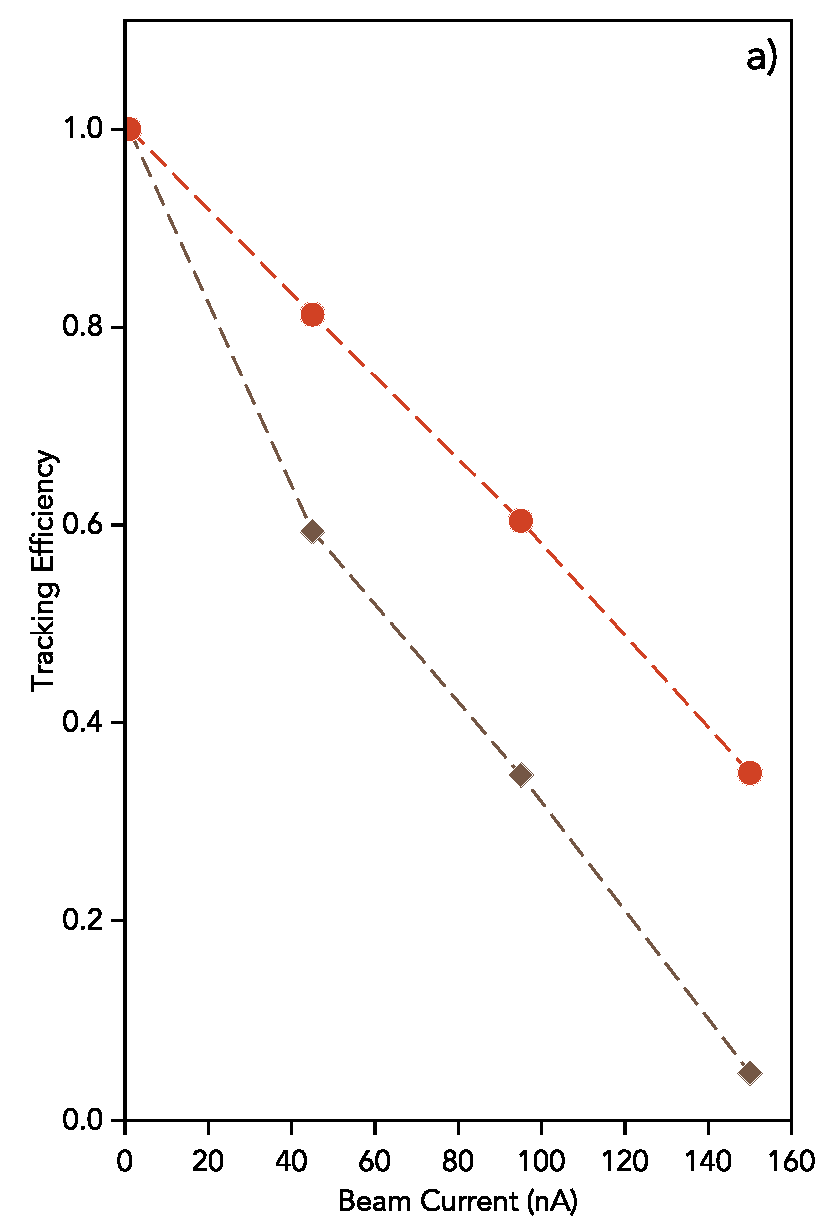
\includegraphics[width=3.1in]{images/figure_phys_scan.pdf}
 %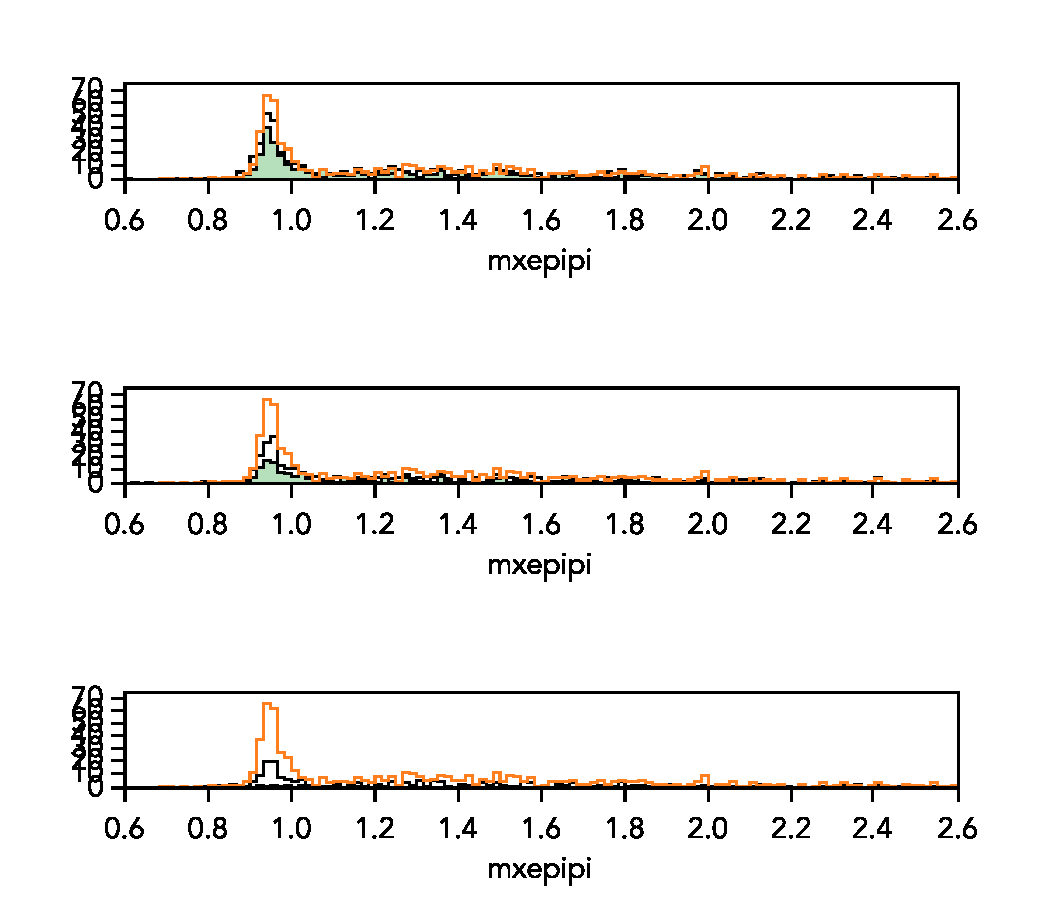
\includegraphics[width=2.5in]{images/figure_phys_conv_compare.pdf}
%\caption {Number of reconstructed protons from missing mass 
%of $H(e e^\prime \pi^+\pi^-)$ for background merged files for 
%$5~nA$, $45~nA$, $95~nA$ and $150~nA$ respectively.}
 %\label{physics::count_raw_dn}
 %\end{center}
%\end{figure}

%On Figure~\ref{physics::conv_dn} (a) the dependence is plotted for both data samples, where the points represent number of events under the proton peak normalized to the number of protons reconstructed by the tracking algorithm before background merging procedure (shown on Figure~\ref{physics::count_raw_dn} in the first column).
%It is evident from the figure that number of reconstructed protons in the de-noised data at $45~nA$ is $37\%$ larger, and the number of reconstructed protons at $95~nA$ in de-noised data sample is $2\%$ larger than in $45~nA$ background merged files. This result has significant implications on future experiments, since the data can be collected much fasted to reach the required statistical significance for given physics program while saving significant amount of money in accelerator operation costs.




